\documentclass{article}
\usepackage{color,soul}
\usepackage{amsmath}
\usepackage{amsfonts} 
\usepackage{eqnarray}
\usepackage{bm}
\usepackage{multirow}
\usepackage{graphicx}
\usepackage{booktabs}
\usepackage{comment}
\usepackage{subcaption}
\usepackage{listings}
\usepackage[margin=0.5in]{geometry}

\title{School of Electrical and Computer Engineering\\
Purdue University, WL, IN, USA}
\author{Nahian Ibn Hasan\\
Email: hasan34@purdue.edu\\
PUID: 0032764564\\
ECE66100 - Computer Vission\\
Fall 2022\\
Homework-4}
\date{\today}

\begin{document}
\maketitle
\section{Objective}
In this homework, we will learn to implement an automated approach for interest point detection and correspondence search for a given pair of images of the same scene.
\section{Theoretical Question}
What is the theoretical reason for why the LoG of an image can be computed as a DoG. Also explain why computing the LoG of an image as a DoG is computationally much more efficient for the same value of $\sigma$.
\subsection{Answer}
Any original image $f(x,y)$ convolved with a gaussian kernel and the LoG operator applied on the resultant smoothed image ($\tilde{f}(x,y)$) can be expressed as $\nabla^2\tilde{f}(x,y)$. We have
\begin{equation}
	\tilde{f}(x,y) = \int_{}^{}\int_{-\infty}^{\infty}f(x',y')g_\sigma(x-x',y-y')dx'dy'
\end{equation}
Partial derivative w.r.t. $\sigma$ provides
\begin{equation}
	\frac{\delta\tilde{f}(x,y,\sigma)}{\delta\sigma} = \sigma\nabla^2\tilde{f}(x,y,\sigma).
\end{equation}
This is the DoG operation. Therefore, multiplying LoG with $\sigma$ will provide the DoG result.
\par From the perspective of digital convolution or discrete convolution, the kernel size for DoG operation is smaller than that of LoG operation. Moreover, DoG operation is possible along single dimension, whereas LoG operations are suitable for 2D data.

\section{Task 1: Harris Corner Detector}
\subsection{Algorithm}
A corner means a pixel near which the gray levels of the image changes signifigicantly in different directions. Assume the x-directed and y-directed first order derivatives are denoted as $d_x$ and $d_y$, respectively, each calculated with a scale $\sigma$. Theese can be calculated by convolving the original image with the following $x$ and $y$ directed Haar filters as-
\begin{equation}
H_x = \begin{bmatrix}
-1&-1&-1&1&1&1\\-1&-1&-1&1&1&1\\-1&-1&-1&1&1&1\\-1&-1&-1&1&1&1\\-1&-1&-1&1&1&1\\-1&-1&-1&1&1&1
\end{bmatrix}
\end{equation}
and
\begin{equation}
H_y = \begin{bmatrix}
1&1&1&1&1&1\\1&1&1&1&1&1\\1&1&1&1&1&1\\-1&-1&-1&-1&-1&-1\\-1&-1&-1&-1&-1&-1\\-1&-1&-1&-1&-1&-1.
\end{bmatrix}
\end{equation}
The above filters are for a scale of $4\sigma;\sigma=1.2$. Here, the kernel size is determined by converting $4\sigma$ to the nearest even integer. Next, we form the $C$ matrix as follows within a local neighbourhood of $5\sigma\times 5\sigma$ around any pixel. Here,
\begin{equation}
	C = \begin{bmatrix}
		\Sigma d_x^2 & \Sigma d_xd_y \\ \Sigma d_xd_y & \Sigma d_y^2
	\end{bmatrix}.
\end{equation}
Next, the trace and determinance of the $C$ matrix is $Tr(C) = \Sigma d_x^2 + \Sigma d_y^2 = \lambda_1 + \lambda_2$ and $det(C) = \Sigma d_x^2 \times \Sigma d_y^2 - (\Sigma d_xd_y)^2 = \lambda_1\lambda_2$, respectively, where $\lambda's$ are the eigenvalues of $C$ matrix and $\lambda_1\geq\lambda_2$. Next the following thresholding criteria is followed-
\begin{equation}
	k = \frac{det(C)}{[Tr(C)]^2} = \frac{\frac{\lambda_2}{\lambda_1}}{(1+\frac{\lambda_2}{\lambda_1})^2}
\end{equation}
\begin{equation}
	R = det(C) - k\times [Tr(C)]^2
\end{equation}
\begin{equation}
	T = 99^{th} \;percentile (R)
\end{equation}
All the pixels with a ratio ($R$) above Threshold ($T$) is considered to be a corner.
\subsection{Correspondence Matrices}
The two sets of interest points from two different images are found from the Harris Corner Detector which are then matched for constructing a one-to-one correspondence relationship for every interest point in the sets. This is done by finding the minimum distance from a specific interest point of one set to all the interest points of the second set. The distance metrics are Sum of Squared Differences (SSD) and Normalized Cross Correlation (NCC). The metrics are defined within an $M\times M$ local window as follows-
\begin{equation}
	SSD = \sum_{i=-M}^{M}\sum_{j=-M}^{M}|f_1(i,j) - f_2(i,j)|^2\\
	NCC = \frac{\sum_{i=-M}^M\sum_{j=-M}^M(f_1(i,j)-\mu_1)(f_2(i,j)-\mu_2)}{\sqrt{\Big[\sum_{i=-M}^M\sum_{j=-M}^M(f_1(i,j)-\mu_1)^2\Big]\Big[\sum_{i=-M}^M\sum_{j=-M}^M(f_2(i,j)-\mu_2)^2}\Big]}.
\end{equation}
Here, $\mu_1$ and $\mu_2$ are the mean gray levels in the espective windows of interest points from two different sets. For our implementation, we have chosen $M=21$
\subsection{SIFT Operator}
All the local extrema of the DoG pyramid ($D(x,y,\sigma)$) are calculated. It corresponds to finding the local maaxima or local minima. $D$ must be known for at least 3 values of $\sigma$ in an octave for the extrema to be identified. The maxima at higher octave have lower resolution than those in the lower octave. So, we apply interpolation using Taylor expansion. The true extrema are thresholded based on these expansions. Next, the orientation is calculated by the gradient of Gaussians. Finally, the descriptor vectors are calculated.
\newpage
\subsection{Interest Points}
\begin{figure}[!htbp]
     \centering
    \captionsetup[subfigure]{labelformat=empty}
    \subcaptionbox{\large\textbf{a}}{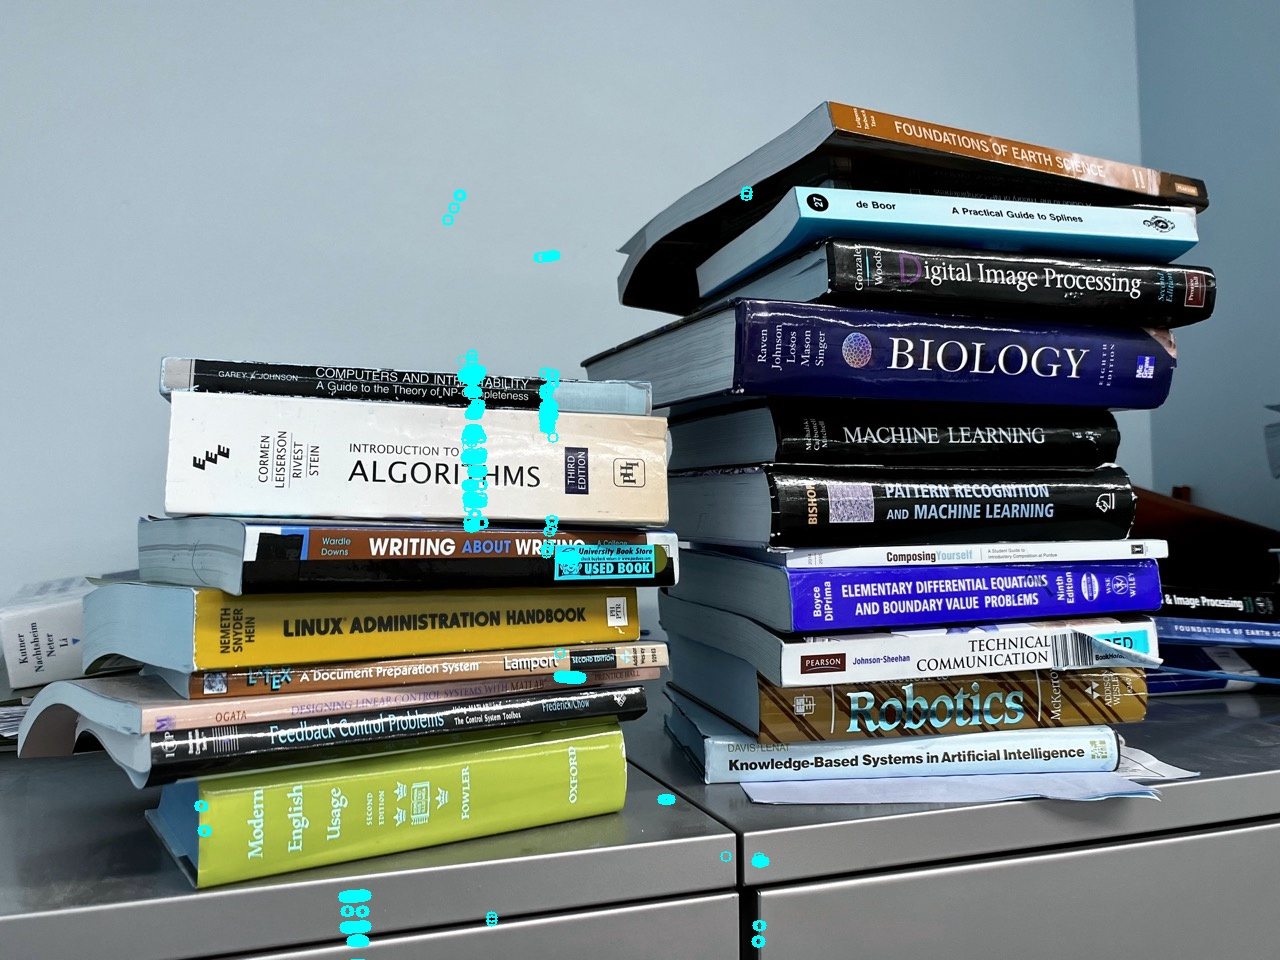
\includegraphics[width=0.45\textwidth]{../Interest_Points_books_1_1.2.jpg}}
    \subcaptionbox{\large\textbf{b}}{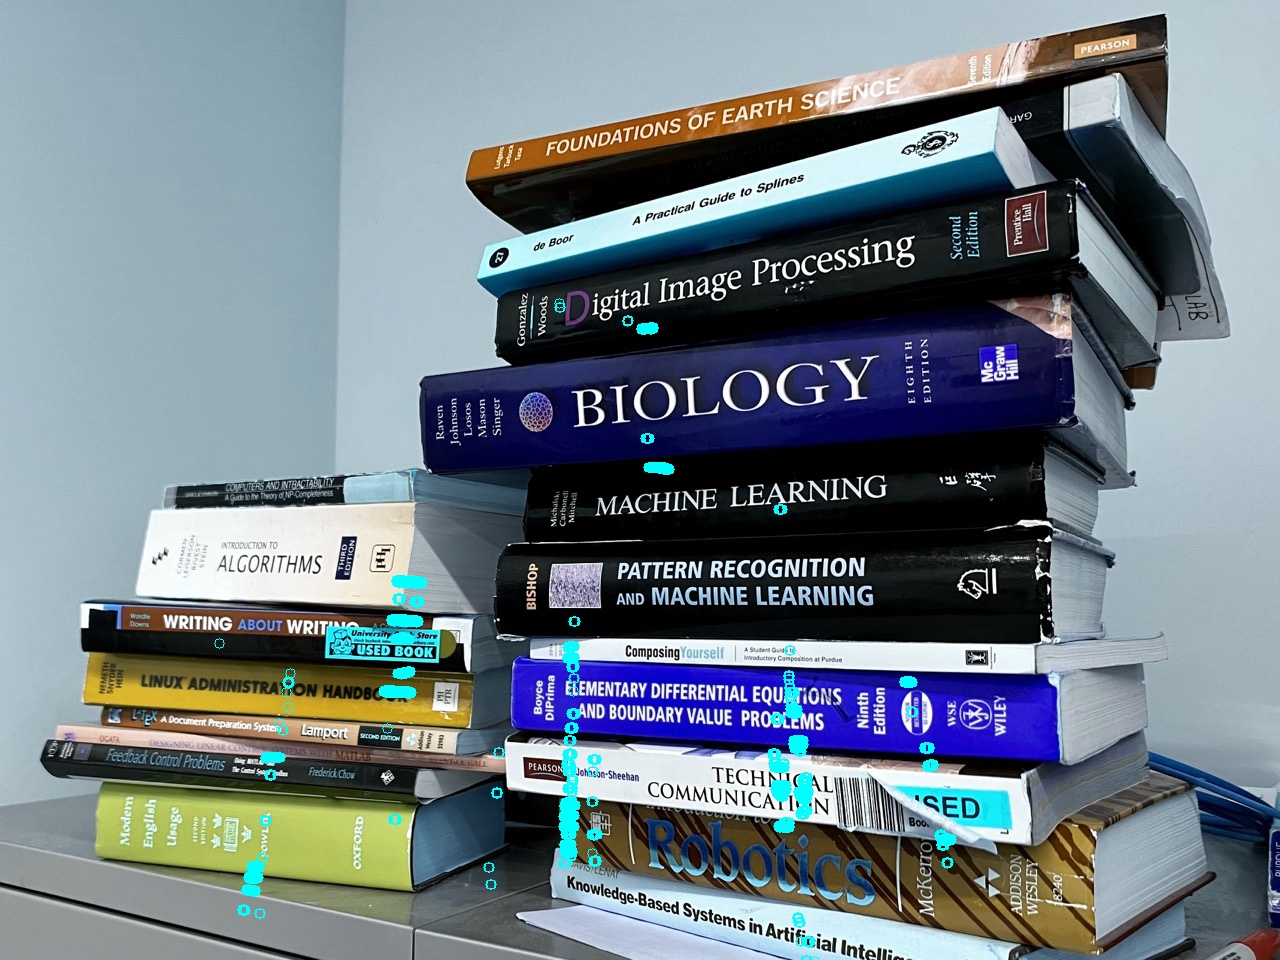
\includegraphics[width=0.45\textwidth]{../Interest_Points_books_2_1.2.jpg}}
    \caption{Interest Points From Harris Corner Point Detector, $\sigma=1.2$}
\end{figure}

\begin{figure}[!htbp]
     \centering
    \captionsetup[subfigure]{labelformat=empty}
    \subcaptionbox{\large\textbf{a}}{\includegraphics[width=0.45\textwidth]{../Interest_Points_fountain_1_1.2.jpg}}
    \subcaptionbox{\large\textbf{b}}{\includegraphics[width=0.45\textwidth]{../Interest_Points_fountain_2_1.2.jpg}}
    \caption{Interest Points From Harris Corner Point Detector, $\sigma=1.2$}
\end{figure}
\newpage
\subsection{Correspondence Between Interest Points}
\begin{figure}[!htbp]
     \centering
    \includegraphics[width=0.9\textwidth]{../Image_Correspondences_SSD_books_1.2.jpg}
    \caption{Interest Points Correspondence, $\sigma=1.2$}
\end{figure}

\begin{figure}[!htbp]
     \centering
    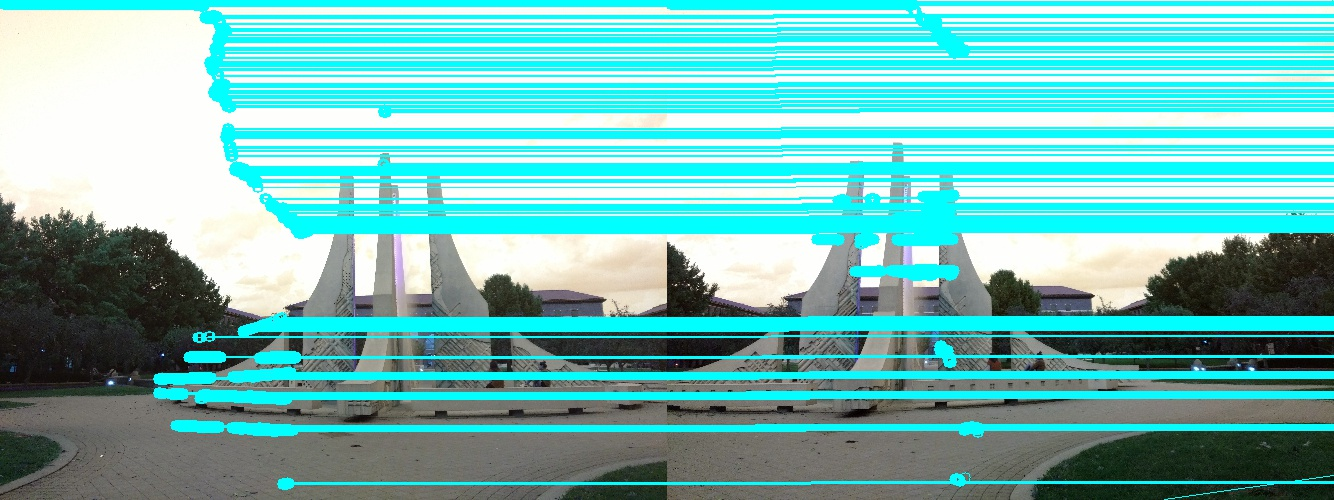
\includegraphics[width=0.9\textwidth]{../Image_Correspondences_SSD_fountain_1.2.jpg}
    \caption{Interest Points Correspondence, $\sigma=1.2$}
\end{figure}
\newpage
\subsection{Interest Point Correspondences for Multiple Scaling}
\begin{figure}[!htbp]
     \centering
    \captionsetup[subfigure]{labelformat=empty}
    \subcaptionbox{\large\textbf{a}}{\includegraphics[width=0.6\textwidth]{../Image_Correspondences_SSD_books_0.8.jpg}}
    \subcaptionbox{\large\textbf{b}}{\includegraphics[width=0.6\textwidth]{../Image_Correspondences_SSD_books_1.2.jpg}}
    \subcaptionbox{\large\textbf{c}}{\includegraphics[width=0.6\textwidth]{../Image_Correspondences_SSD_books_1.6.jpg}}
    \subcaptionbox{\large\textbf{d}}{\includegraphics[width=0.6\textwidth]{../Image_Correspondences_SSD_books_2.0.jpg}}
    \caption{Interest Points Correspondence for a scale($\sigma$) of 0.8 (a),1.2(b),1.6(c) and 2.0(d)}
\end{figure}

\newpage
\begin{figure}[!htbp]
     \centering
    \captionsetup[subfigure]{labelformat=empty}
    \subcaptionbox{\large\textbf{a}}{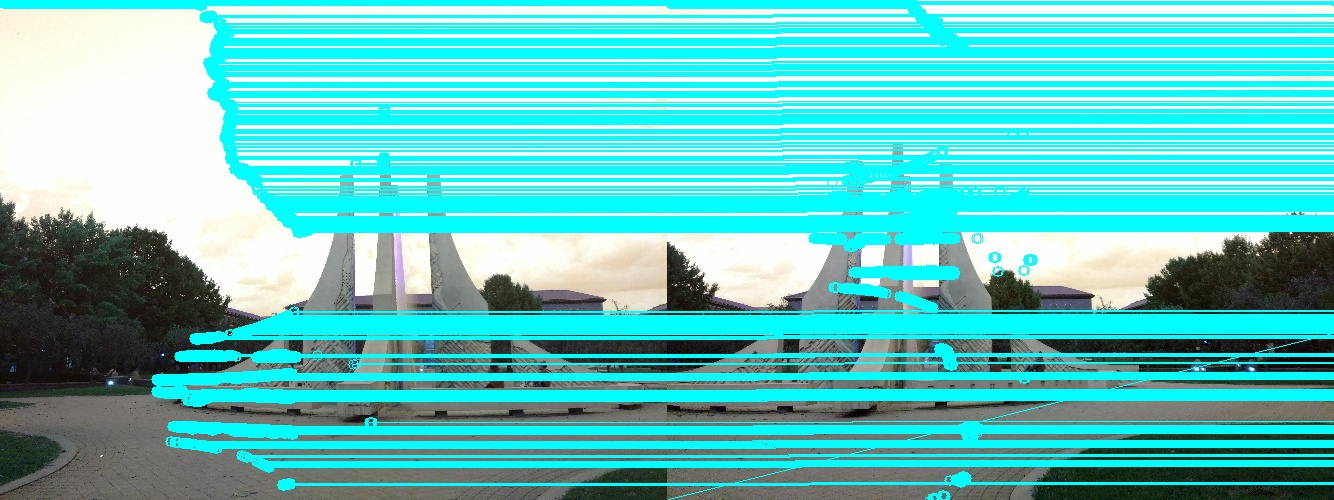
\includegraphics[width=0.6\textwidth]{../Image_Correspondences_SSD_fountain_0.8.jpg}}
    \subcaptionbox{\large\textbf{b}}{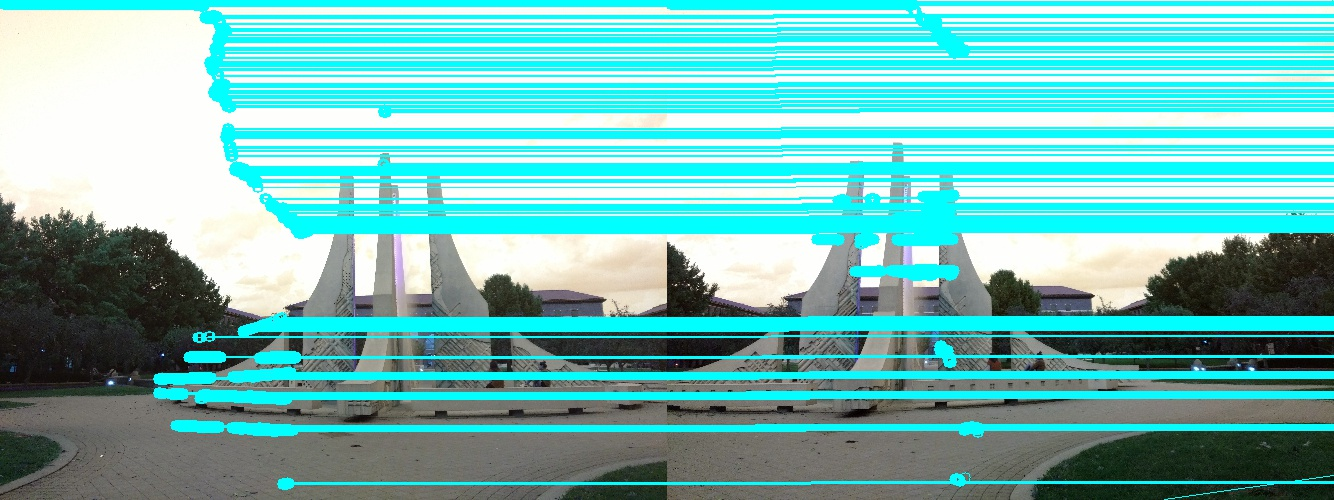
\includegraphics[width=0.6\textwidth]{../Image_Correspondences_SSD_fountain_1.2.jpg}}
    \subcaptionbox{\large\textbf{c}}{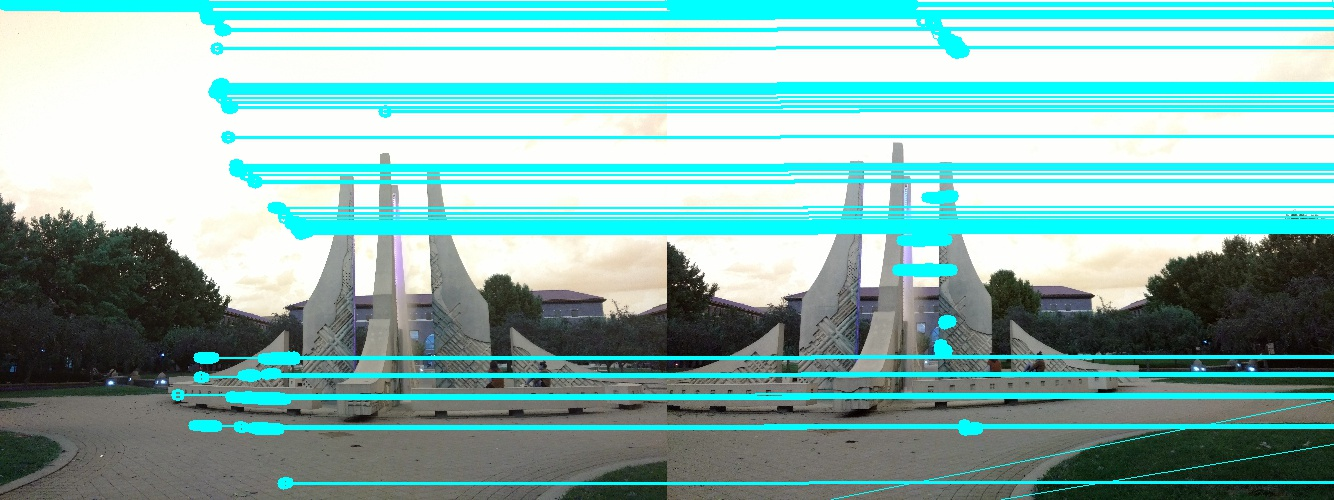
\includegraphics[width=0.6\textwidth]{../Image_Correspondences_SSD_fountain_1.6.jpg}}
    \subcaptionbox{\large\textbf{d}}{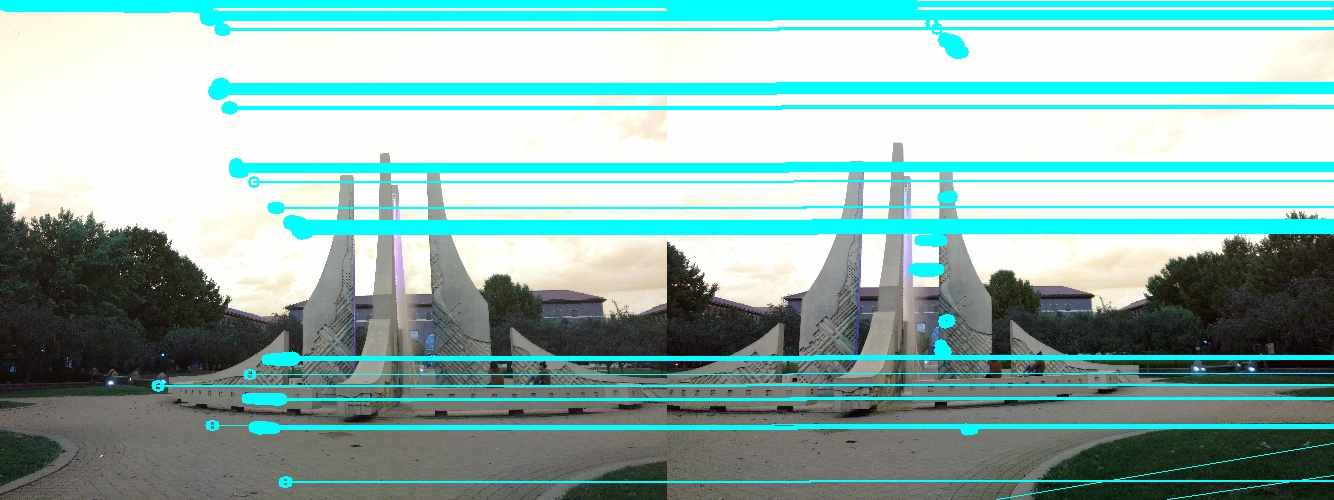
\includegraphics[width=0.6\textwidth]{../Image_Correspondences_SSD_fountain_2.0.jpg}}
    \caption{Interest Points Correspondence for a scale($\sigma$) of 0.8 (a),1.2(b),1.6(c) and 2.0(d)}
\end{figure}
\newpage
\section{OpenCV SIFT Operator Output}
\begin{figure}[!htbp]
     \centering
    \captionsetup[subfigure]{labelformat=empty}
    \subcaptionbox{\large\textbf{a}}{\includegraphics[width=0.9\textwidth]{../opencv_correspondences_books_1.2.jpg}}
    \subcaptionbox{\large\textbf{b}}{\includegraphics[width=0.9\textwidth]{../opencv_correspondences_fountain_1.2.jpg}}
    \caption{Interest Points Correspondence from OpenCV SIFT operation}
\end{figure}

\newpage
\section{Superglue and Superpoint Output}
\begin{figure}[!htbp]
     \centering
    \captionsetup[subfigure]{labelformat=empty}
    \subcaptionbox{\large\textbf{a}}{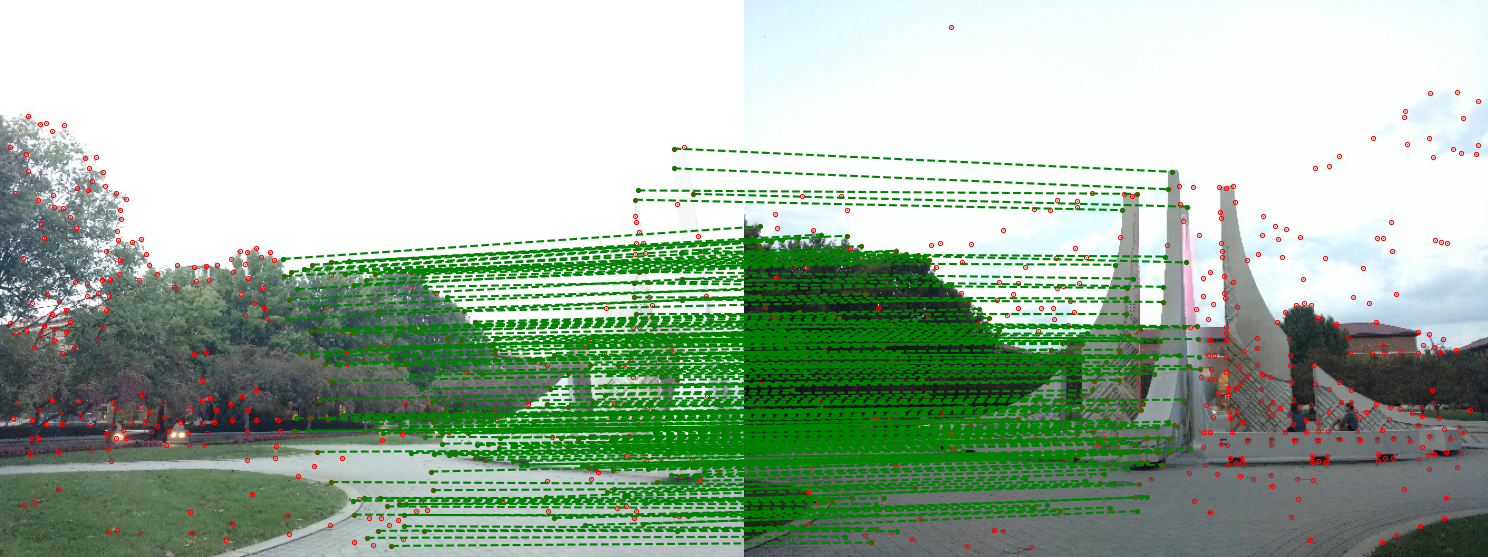
\includegraphics[width=0.55\textwidth]{../1_and_2_superglue_matches.png}}
    \subcaptionbox{\large\textbf{b}}{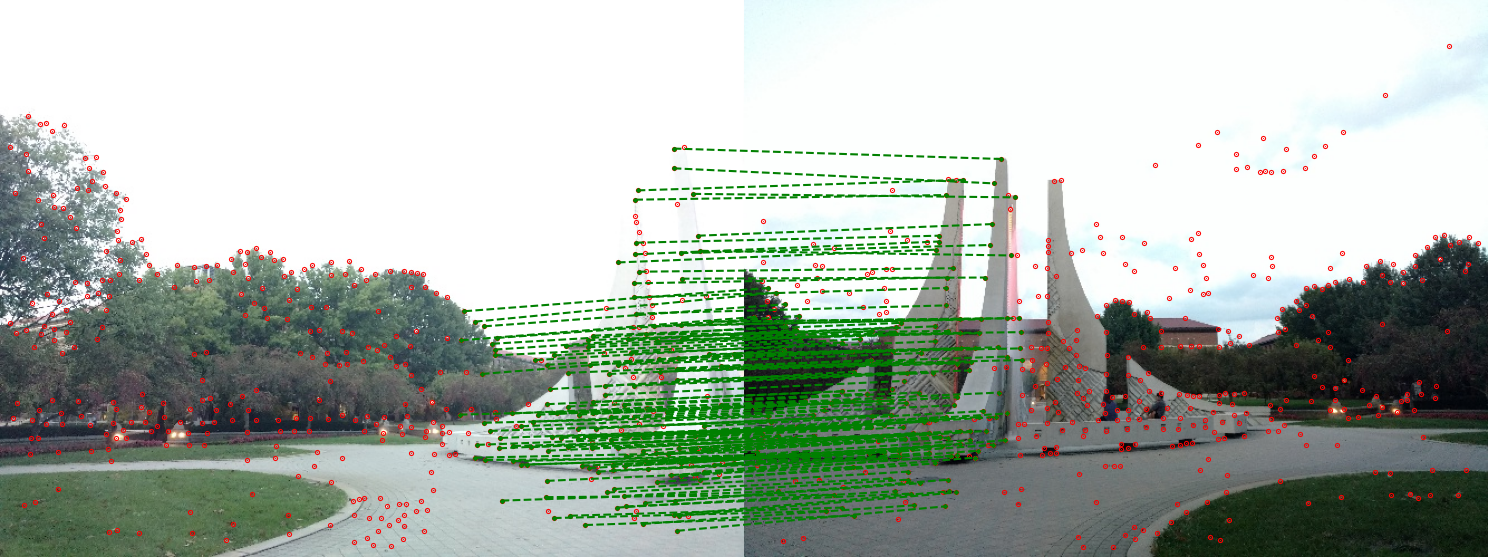
\includegraphics[width=0.55\textwidth]{../1_and_3_superglue_matches.png}}
    \subcaptionbox{\large\textbf{c}}{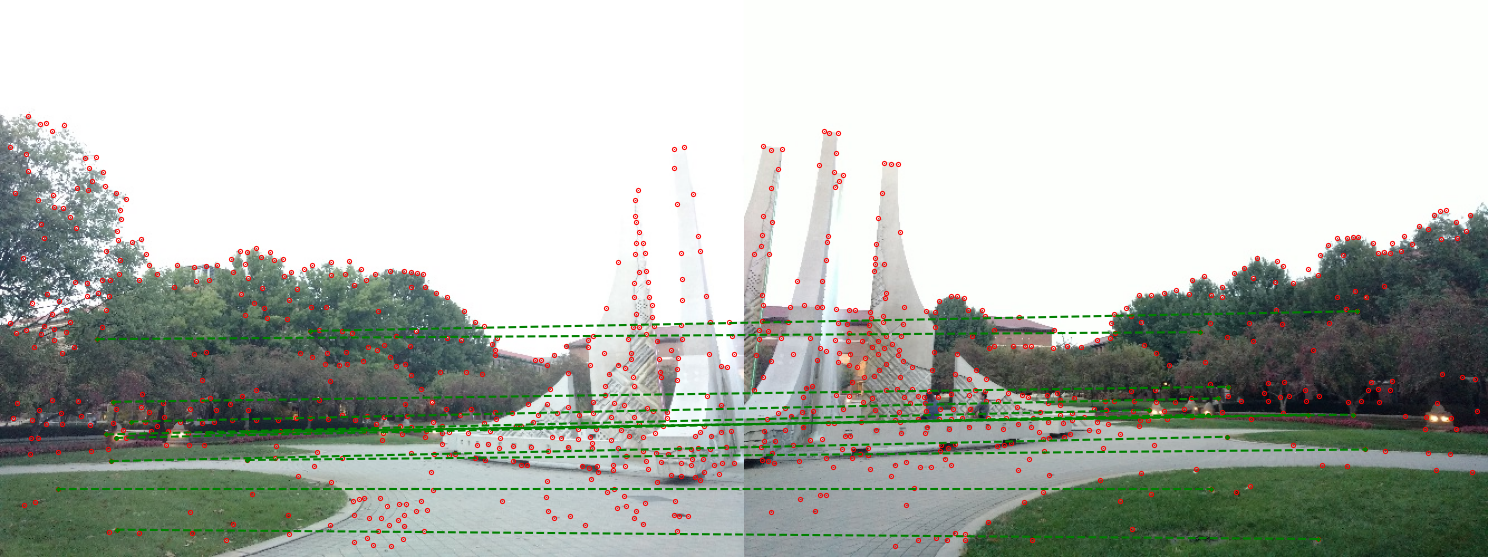
\includegraphics[width=0.55\textwidth]{../1_and_4_superglue_matches.png}}
    \subcaptionbox{\large\textbf{d}}{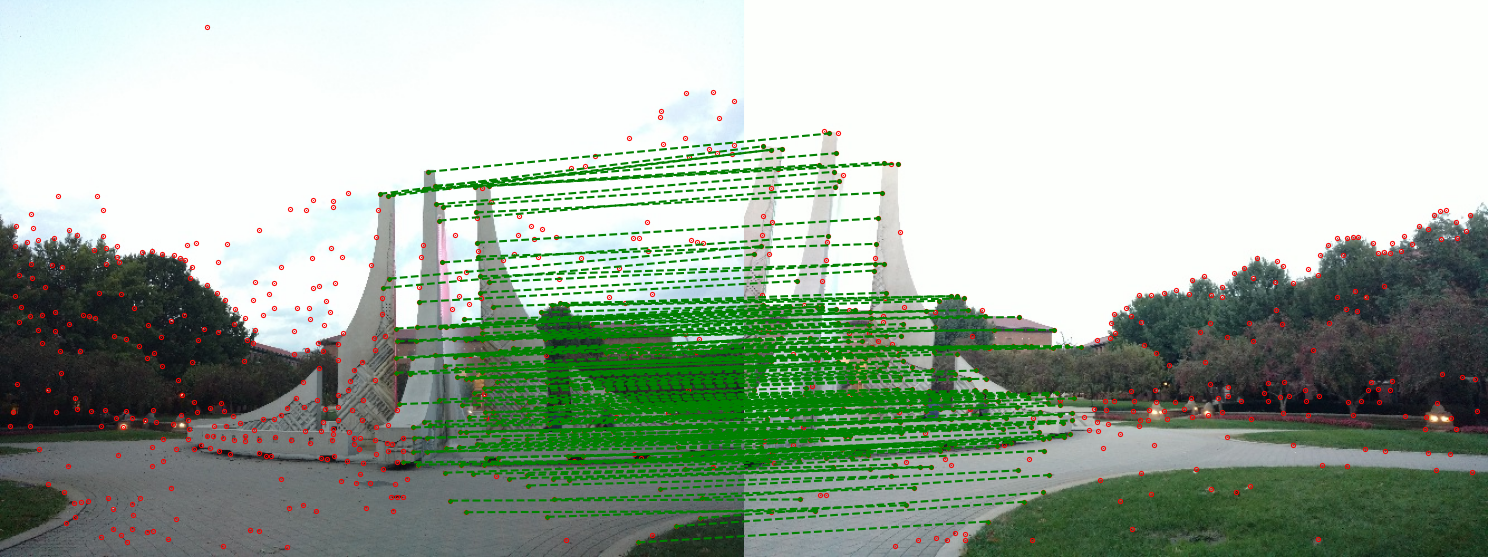
\includegraphics[width=0.55\textwidth]{../2_and_4_superglue_matches.png}}
    \subcaptionbox{\large\textbf{e}}{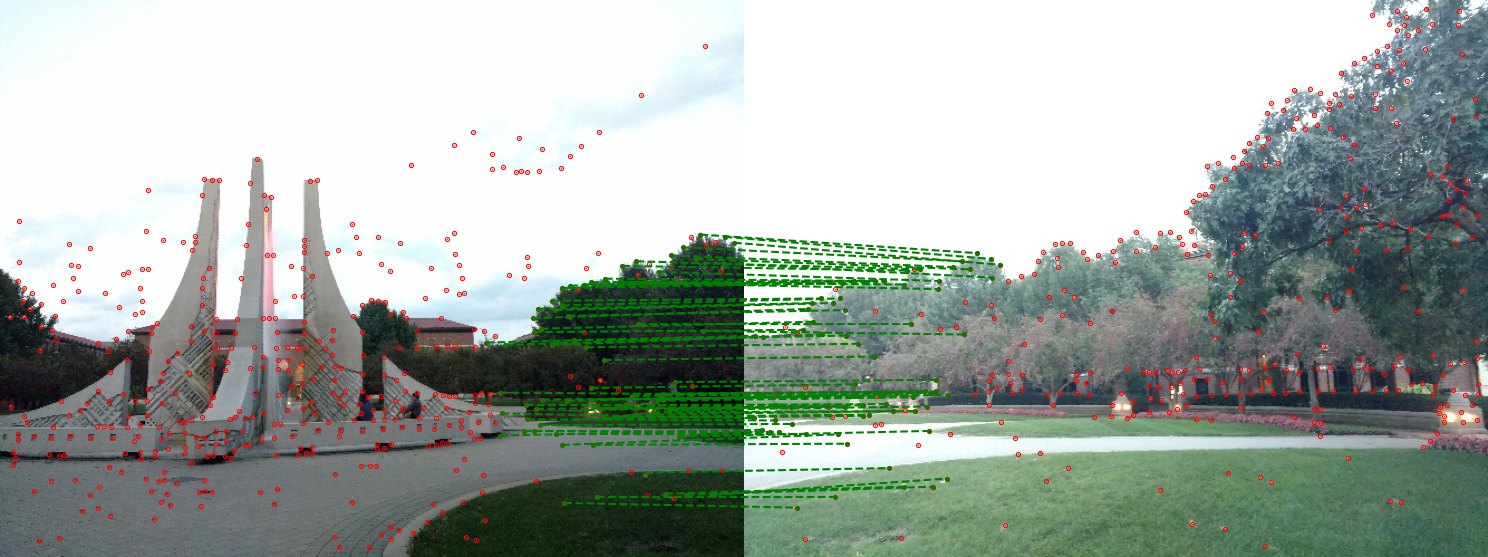
\includegraphics[width=0.55\textwidth]{../3_and_5_superglue_matches.png}}
    \caption{Interest Points Correspondence from Superglue and Superpoint platforms}
\end{figure}


\section{Interest Point Correspondences for Custom Images}
\begin{figure}[!htbp]
     \centering
    \captionsetup[subfigure]{labelformat=empty}
    \subcaptionbox{\large\textbf{a}}{\includegraphics[width=0.6\textwidth]{../Image_Correspondences_SSD_custom_pair_1_0.8.jpg}}
    \subcaptionbox{\large\textbf{b}}{\includegraphics[width=0.6\textwidth]{../Image_Correspondences_SSD_custom_pair_1_1.2.jpg}}
    \subcaptionbox{\large\textbf{c}}{\includegraphics[width=0.6\textwidth]{../Image_Correspondences_SSD_custom_pair_1_1.6.jpg}}
    \subcaptionbox{\large\textbf{d}}{\includegraphics[width=0.6\textwidth]{../Image_Correspondences_SSD_custom_pair_1_2.0.jpg}}
    \caption{Interest Points Correspondence for a scale ($\sigma$) of 0.8 (a),1.2(b),1.6(c) and 2.0(d) in custom pair image pair 1}
\end{figure}

\begin{figure}[!htbp]
     \centering
    \captionsetup[subfigure]{labelformat=empty}
    \subcaptionbox{\large\textbf{a}}{\includegraphics[width=0.6\textwidth]{../Image_Correspondences_SSD_custom_pair_2_0.8.jpg}}
    \subcaptionbox{\large\textbf{b}}{\includegraphics[width=0.6\textwidth]{../Image_Correspondences_SSD_custom_pair_2_1.2.jpg}}
    \subcaptionbox{\large\textbf{c}}{\includegraphics[width=0.6\textwidth]{../Image_Correspondences_SSD_custom_pair_2_1.6.jpg}}
    \subcaptionbox{\large\textbf{d}}{\includegraphics[width=0.6\textwidth]{../Image_Correspondences_SSD_custom_pair_2_2.0.jpg}}
    \caption{Interest Points Correspondence for a scale ($\sigma$) of 0.8 (a),1.2(b),1.6(c) and 2.0(d) in custom pair image pair 2}
\end{figure}

\section{Remarks}
It seems the source image pair have high impact on the accuracy of the corresondence among interest points. For example, custom  image pair 1 had a hard time in finding the proper harris corner match.\\
Also, the Superpoint+Superglue pipeline seems to provide amazing accuracy in the correspondence. The performance seems almost equal (in some cases better than) to openCV SIFT operation.\\
The parameters for efficient feature extraction are mentioned in the theory section. Also, the percentile thresholds for each different scenario are mentioned in the main file of the source code. Almost for all of the cases, having a 99 percentile threshold was enough for finding enough number of corner point candidates.
\newpage
\subsection{Source Code}
\subsubsection{main.py}
\begin{lstlisting}[language=Python]
import os
import numpy as np
import matplotlib.pyplot as plt
from PIL import Image
import matplotlib.image as mpimg
import harris_corner_detector as HCD
import correspondence_metrics as CM
import time
import cv2


def opencv_interest_points(im_path,name):
	img = cv2.imread(im_path)
	gray= cv2.cvtColor(img,cv2.COLOR_BGR2GRAY)
	sift = cv2.SIFT_create()
	kp,des = sift.detectAndCompute(gray,None)
	img=cv2.drawKeypoints(gray,kp,img)
	cv2.imwrite('sift_keypoints_'+name+'.jpg',img)
	return img,kp,des

def opencv_correspondence(img_1,kp_1,des_1,img_2,kp_2,des_2,name,N):
	#N 	: how many correspondences to be kept
	bf = cv2.BFMatcher(cv2.NORM_L1, crossCheck=True)# create BFMatcher object
	matches = bf.match(des_1,des_2)# Match descriptors.
	matches = sorted(matches, key = lambda x:x.distance)# Sort them in the order of their distance.
	img3 = cv2.drawMatches(img_1,kp_1,img_2,kp_2,matches[:N], None,flags=2)# Draw first 10 matches.
	cv2.imwrite('opencv_correspondences_'+name+'.jpg',img3)

def plot_interest_points(Im,indexes,name,scale):
	for ix in range(0,indexes.shape[0]):
		cv2.circle(Im,indexes[ix,:],5,(255, 255, 0),1)
	cv2.imwrite('Interest_Points_'+name+'_'+str(scale)+'.jpg',Im)

def corner_detection_image_pairs(Im_1_path,Im_2_path,name_1,name_2,Th,scale):
	Im_1 = mpimg.imread(Im_1_path)
	Im_2 = mpimg.imread(Im_2_path)
	print("Image Files Read")

	start_time = time.time()
	[corner_indexes_1,Th_1] = HCD.harris_detector(Im_1,scale,Th)
	print("Interest Points Detected for "+name_1)
	end_time = time.time()
	[corner_indexes_2,Th_2] = HCD.harris_detector(Im_2,scale,Th)
	print("Interest Points Detected for "+name_2)
	print('Required Time for Harris Corner Detection Algorithm = ',str(end_time-start_time))
	plot_interest_points(Im_1,corner_indexes_1,name_1,scale)
	plot_interest_points(Im_2,corner_indexes_2,name_2,scale)
	print("Interest Points Plotted")
	correspondences_SSD = CM.Sum_of_Squared_Differences(Im_1,Im_2,corner_indexes_1,corner_indexes_2,21)
	correspondences_NCC = CM.Normalized_Cross_Correlations(Im_1,Im_2,corner_indexes_1,corner_indexes_2,21)
	CM.plot_correspondences(Im_1,Im_2,correspondences_SSD,corner_indexes_1,corner_indexes_2,10000,'SSD_'+name_1[:-2]+'_'+str(scale))
	CM.plot_correspondences(Im_1,Im_2,correspondences_NCC,corner_indexes_1,corner_indexes_2,10000,'NCC_'+name_1[:-2]+'_'+str(scale))


def main():
	scales=[0.8,1.2,1.6,2.0]

	im_1 = './HW4-Images/Figures/books_1.jpeg'
	im_2 = './HW4-Images/Figures/books_2.jpeg'
	for scale in scales:
		corner_detection_image_pairs(im_1,im_2,'books_1','books_2',99.99,scale)
		if scale==1.2:
			[img_1,kp_1,des_1] = opencv_interest_points(im_1,'books_1_'+str(scale))
			[img_2,kp_2,des_2] = opencv_interest_points(im_2,'books_2_'+str(scale))
			opencv_correspondence(img_1,kp_1,des_1,img_2,kp_2,des_2,'books_'+str(scale),10)
	
	im_1 = './HW4-Images/Figures/fountain_1.jpg'
	im_2 = './HW4-Images/Figures/fountain_2.jpg'
	for scale in scales:
		corner_detection_image_pairs(im_1,im_2,'fountain_1','fountain_2',99,scale)
		if scale==1.2:
			[img_1,kp_1,des_1] = opencv_interest_points(im_1,'fountain_1'+str(scale))
			[img_2,kp_2,des_2] = opencv_interest_points(im_2,'fountain_2'+str(scale))
			opencv_correspondence(img_1,kp_1,des_1,img_2,kp_2,des_2,'fountain_'+str(scale),10)

	im_1 = './HW4-Images/Figures/custom_pair_1_1.jpg'
	im_2 = './HW4-Images/Figures/custom_pair_1_2.jpg'
	for scale in scales:
		corner_detection_image_pairs(im_1,im_2,'custom_pair_1_1','custom_pair_1_2',99.95,scale)

	im_1 = './HW4-Images/Figures/custom_pair_2_1.jpg'
	im_2 = './HW4-Images/Figures/custom_pair_2_2.jpg'
	for scale in scales:
		corner_detection_image_pairs(im_1,im_2,'custom_pair_2_1','custom_pair_2_2',99.99,scale)
	
main()
\end{lstlisting}
\subsubsection{harris\_corner\_detector.py}
\begin{lstlisting}[language=Python]
import os
import numpy as np


def haar_kernel(sigma):
	N = int(np.ceil(4*sigma))
	if N%2 == 1:
		N = N+1
	h_x = np.ones((N,N))
	h_y = np.ones((N,N))
	h_x[:,0:int(N/2)]=-1
	h_y[int(N/2):-1,:] = -1
	return h_x,h_y,N

def convolution(image,filter,padding_mode='constant'):
	[height,width] = image.shape
	N = filter.shape[0]
	result = np.zeros((height,width))
	#Pad the image for handling corner operations
	image = np.pad(image,((int(N/2),int(N/2)-1),(int(N/2),int(N/2)-1)),mode=padding_mode)
	for i in range(int(N/2),image.shape[0]-(int(N/2)-1)):
		for j in range(int(N/2),image.shape[1]-(int(N/2)-1)):
			im_neighbour = image[i-int(N/2):i+int(N/2),j-int(N/2):j+int(N/2)]
			result[i-int(N/2),j-int(N/2)] = np.sum(np.multiply(im_neighbour,filter))
	#print(np.unique(result.flatten()))
	return result

def harris_detector(Im,sigma,Th):
	#Im = input image
	#sigma  = Scale factor
	#Th = Threshold percentile
	#Outputs:
	#corners : binary image of same shape as I with 1=corners, 0 = not corners
	#ratios : determinant(C)/Trace(C)^2, can be used later for thresholding with a separate threshold
	#define kernels

	Im = np.array(Im)
	if len(Im.shape)>2:
		Im = Im[:,:,0]
	Im = Im/255

	[h_x,h_y,N] = haar_kernel(sigma)
	dx = convolution(Im,h_x)
	dy = convolution(Im,h_y)
	dx2 = np.multiply(dx,dx)
	dy2 = np.multiply(dy,dy)
	dxdy = np.multiply(dx,dy)

	N_sum = int(np.ceil(5*sigma))
	if N_sum%2 == 1:
		N_sum = N_sum+1
	sum_filter = np.ones((N_sum,N_sum))
	dx2 = convolution(dx2,sum_filter)
	dy2 = convolution(dy2,sum_filter)
	dxdy = convolution(dxdy,sum_filter)
	Tr_C = dx2 + dy2
	det_C = np.multiply(dx2,dy2) - np.multiply(dxdy,dxdy)

	k_tmp = det_C/np.square(Tr_C)
	k_tmp[np.isnan(k_tmp)] = 0
	k = np.sum(k_tmp)/(Im.shape[0]*Im.shape[1])
	R = det_C - k*np.square(Tr_C)
	Th = np.percentile(R, Th)
	print('R_threshold = ',Th)
	corner_indexes = np.argwhere(R>=Th)
	print('Number of corners = ',corner_indexes.shape[0])

	return corner_indexes,Th
\end{lstlisting}
\subsubsection{correspondence\_metrics.py}
\begin{lstlisting}[language=Python]
import numpy as np
import cv2

def Sum_of_Squared_Differences(Im_1,Im_2,corner_indexes_1,corner_indexes_2,N,padding_mode='constant'):
	#N	: N*N neighbourhood
	I_1 = np.pad(Im_1,((int(N/2),int(N/2)),(int(N/2),int(N/2)),(0,0)),mode=padding_mode)
	I_2 = np.pad(Im_2,((int(N/2),int(N/2)),(int(N/2),int(N/2)),(0,0)),mode=padding_mode)
	Best_Matches = np.zeros((corner_indexes_1.shape[0],1))
	for s1 in range(0,corner_indexes_1.shape[0]):
		SSD = np.zeros((corner_indexes_2.shape[0],1))
		i = corner_indexes_1[s1,0]
		j = corner_indexes_1[s1,1]
		ix = i+int(N/2)
		jx = j+int(N/2)
		f_1 = I_1[ix-int(N/2):ix+int(N/2),jx-int(N/2):jx+int(N/2),0]
		for s2 in range(0,corner_indexes_2.shape[0]):
			i = corner_indexes_2[s2,0]
			j = corner_indexes_2[s2,1]
			ix = i+int(N/2)
			jx = j+int(N/2)
			f_2 = I_2[ix-int(N/2):ix+int(N/2),jx-int(N/2):jx+int(N/2),0]
			SSD[s2,0] = np.sum(np.square(f_1 - f_2))
		Best_Matches[s1,0] = np.argsort(SSD)[0]
	return Best_Matches

def Normalized_Cross_Correlations(Im_1,Im_2,corner_indexes_1,corner_indexes_2,N,padding_mode='constant'):
	#N	: N*N neighbourhood
	I_1 = np.pad(Im_1,((int(N/2),int(N/2)),(int(N/2),int(N/2)),(0,0)),mode=padding_mode)
	I_2 = np.pad(Im_2,((int(N/2),int(N/2)),(int(N/2),int(N/2)),(0,0)),mode=padding_mode)
	Best_Matches = np.zeros((corner_indexes_1.shape[0],1))

	for s1 in range(0,corner_indexes_1.shape[0]):
		i = corner_indexes_1[s1,0]
		j = corner_indexes_1[s1,1]
		ix = i+int(N/2)
		jx = j+int(N/2)
		f_1 = I_1[ix-int(N/2):ix+int(N/2),jx-int(N/2):jx+int(N/2),0]
		m_1 = np.mean(I_1[ix-int(N/2):ix+int(N/2),jx-int(N/2):jx+int(N/2),0])
		NCC = np.zeros((corner_indexes_2.shape[0],1))
		for s2 in range(0,corner_indexes_2.shape[0]):
			i = corner_indexes_2[s2,0]
			j = corner_indexes_2[s2,1]
			ix = i+int(N/2)
			jx = j+int(N/2)
			f_2 = I_2[ix-int(N/2):ix+int(N/2),jx-int(N/2):jx+int(N/2),0]
			m_2 = np.mean(I_2[ix-int(N/2):ix+int(N/2),jx-int(N/2):jx+int(N/2),0])
			num = np.sum(np.multiply((f_1-m_1),(f_2-m_2)))
			den = np.sqrt(np.multiply(np.sum(np.square(f_1-m_1)),np.sum(np.square(f_2-m_2))))
			if den != 0:
				NCC[s2,0] = num/den
		Best_Matches[s1,0] = np.argsort(NCC)[0]

	return Best_Matches

def plot_correspondences(I_1,I_2,Best_Matches,corner_indexes_1,corner_indexes_2,M,name):
	#M	: how many correspondences to show
	CI = np.concatenate((I_1,I_2),axis=1)
	im_width = I_1.shape[1]
	for ix in range(0,min(M,corner_indexes_1.shape[0])):
		points_1 = tuple([corner_indexes_1[ix,1],corner_indexes_1[ix,0]])
		pt2 = corner_indexes_2[int(Best_Matches[ix]),:]
		points_2 = tuple([pt2[1]+im_width,pt2[0]])
		#print(points_1,'---',Best_Matches[ix,],'----',points_2,'----',im_width)
		cv2.circle(CI,points_1,5,(255, 255, 0),1)
		cv2.circle(CI,points_2,5,(255, 255, 0),1)
		cv2.line(CI,points_1,points_2,(255, 255, 0),1)
	cv2.imwrite('Image_Correspondences_'+name+'.jpg',CI)
\end{lstlisting}
\end{document}
